
\documentclass{beamer}

\usepackage[utf8]{inputenc}
\usepackage{amsmath}

\usepackage{wrapfig}
\usepackage{caption}
\usepackage{tcolorbox}
\usepackage{tabulary}
\usepackage{cite}

\input{test}

\expandafter\def\expandafter\quote\expandafter{\quote\small}

\usefonttheme[onlymath]{serif}

\usetheme{Copenhagen}
\usecolortheme{beaver}

\title{Künstliche Intelligenz}
\author{Lennart Wilde}
\institute{Nationales Patentrecht}
\date{18. Mai 2020}

\renewcommand{\figurename}{Fig.}

%%%%%%%%%%%%%%%%%%%%%%%%%%%%%%%%%% SEITENZAHLEN AUF  FOLIE %%%%%%%%%%%%%%%%%%%%%%%%%%%%%

\defbeamertemplate{footline}{centered page number}
{%
  \hspace*{\fill}%
  \usebeamercolor[fg]{page number in head/foot}%
  \usebeamerfont{page number in head/foot}%
  \insertpagenumber\,/\,\insertpresentationendpage%
  \hspace*{\fill}\vskip2pt%
}

\setbeamertemplate{footline}[centered page number]

\beamertemplatenavigationsymbolsempty

%%%%%%%%%%%%%%%%%%%%%%%%%%%%%%%%%%%%%%%%%%%%%%%%%%%%%%%%%%%%%%%%%%%%%%%%%%%%%%%%%%%%%%

%%%%%%%%%%%%%%%%%%%%%%%%%% ANDERER ITEMIZE STIL %%%%%%%%%%%%%%%%%%%%%%%%%%%%%%%%%%%%%%%

\setbeamertemplate{itemize items}[default]
\setbeamertemplate{enumerate items}[default]

%%%%%%%%%%%%%%%%%%%%%%%%%%%%%%%%%%%%%%%%%%%%%%%%%%%%%%%%%%%%%%%%%%%%%%%%%%%%%%%%%%%%%%
\begin{document}
    \frame{\titlepage}

    \begin{frame}[t]{Eine kleine Geschichte der KI}
      \only<1>{
        \begin{center}
          Menschen waren schon immer von der Idee einer selbst geschffenen Intelligenz fasziniert\\
          \vspace{1cm}

          In beinahe jedem Zeitalter gab es neue Überlegungen und Erfindungen die dem Menschen das Denken abnehmen sollten\\
        \end{center}
      }

      \only<2>{
      \framesubtitle{Der Traum der KI}
        \centering
        \begin{figure}
          \begin{minipage}{0.59 \textwidth}
            \textbf{Beispiel:}\\
            Der Mechanische Schachspieler
            \begin{itemize}
              \item gebaut im Jahr 1769
              \item schien sebstständig Schach zu spielen
            \end{itemize}
          \end{minipage}
          \begin{minipage}{0.39 \textwidth}
            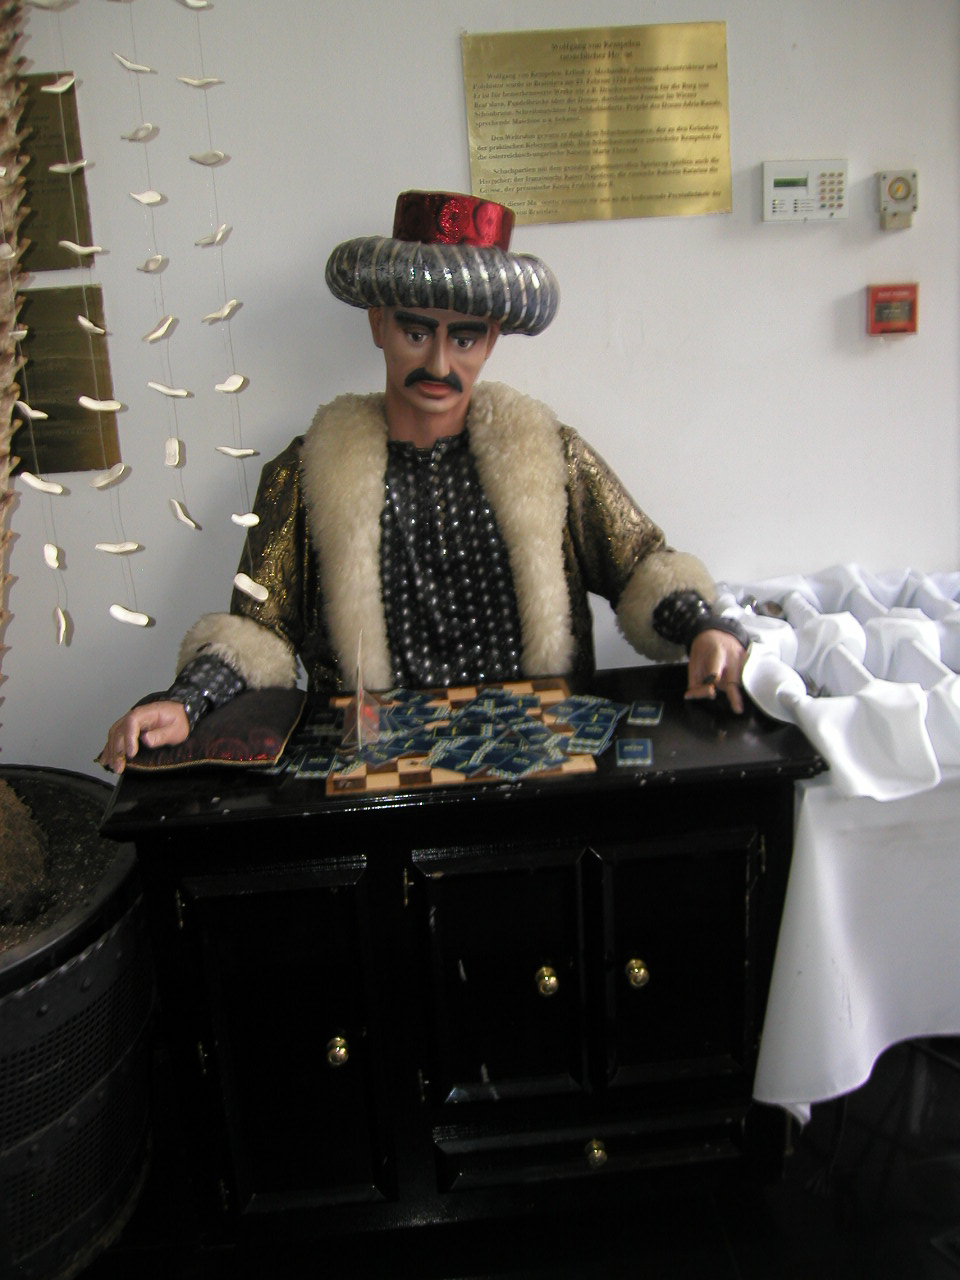
\includegraphics[width = \textwidth]{Pictures/Schachtuerke}
            \caption{\footnotesize Quelle: Von Schorle - Eigenes Werk, CC BY-SA 3.0}
          \end{minipage}
        \end{figure}
      }

      \only<3>{
      \framesubtitle{Der Traum der KI}
        \centering
        \begin{figure}
          \begin{minipage}{0.59 \textwidth}
            \textbf{Beispiel:}\\
            Der Mechanische Schachspieler
            \begin{itemize}
              \item gebaut im Jahr 1769
              \item schien sebstständig Schach zu spielen
              \item war zwar eine Schwindelei, \textbf{aber} trotzdem sehr populär
            \end{itemize}
          \end{minipage}
          \begin{minipage}{0.39 \textwidth}
            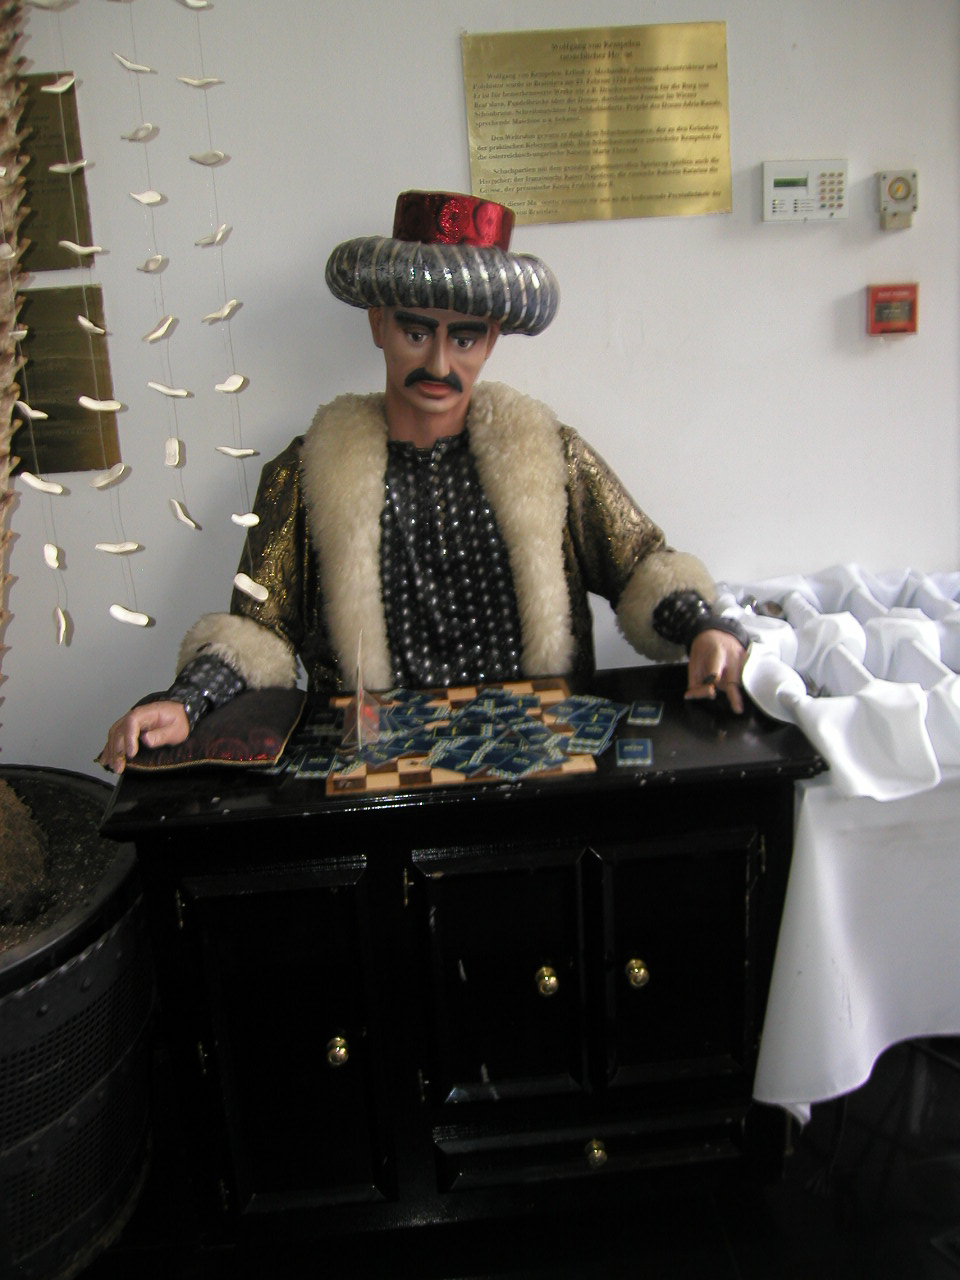
\includegraphics[width = \textwidth]{Pictures/Schachtuerke}
            \caption{\footnotesize Quelle: Von Schorle - Eigenes Werk, CC BY-SA 3.0}
          \end{minipage}
        \end{figure}
      }

      \only<4>{
        \framesubtitle{Timeline}
        \begin{center}
        \vspace{-0.2cm}
          \begin{timeline}{1642}{1950}{0.2 \paperwidth}{0.2 \paperwidth}{0.6 \paperwidth}{0.7 \paperheight}

            \entry{1642}{Mechanischer Rechner}
            \entry{1769}{Mechanischer Schachspieler}
            \entry{1818}{Frankenstein; or the modern Prometheus}
            \entry{1863}{Evolutionstheorie der Maschinen}
            \plainentry{1941}{Erster Elektronischer Computer}
            \entry{1950}{Turing Test}

          \end{timeline}
        \end{center}

      }

      \only<5>{
        \framesubtitle{Timeline}
        \vspace{-0.2cm}
        \begin{center}
          \begin{timeline}{1980}{2018}{0.2 \paperwidth}{0.2 \paperwidth}{0.6 \paperwidth}{0.7 \paperheight}

            \entry{1986}{Erste Selbstfahrende Kfz}
            \entry{1989}{Entwicklung von MOS-Technologie}
            \entry{1995}{No Hands across America}
            \entry{1997}{Deep Blue}
            \entry{2009}{Erste autonome Fahrzeuge von Google}
            \entry{2011}{Siri und ähnliche Sprachassistenten}
            \entry{2016}{AlphaGo schlägt Lee Sedol 4-1}
            \entry{2018}{\footnotesize AlphaGo Zero lernt innerhalb von 4 Stunden Schach}

          \end{timeline}
        \end{center}

      }

    \end{frame}
    %--- Next Frame ---%

    \begin{frame}{Was ist Künstliche Intelligenz?}
      \only<1>{
        \framesubtitle{Definition?}
        \begin{itemize}
          \item Allein schon \textbf{Intelligenz} zu definieren ist schwierig.
        \end{itemize}
      }

      \only<2>{
        \framesubtitle{Lösungsansätze}

        Häufig verwendet: \begin{quote}
                            \textbf{Künstliche Intelligenz} beschreibt den Versuch bestimmte Entscheidungsstrukturen des Menschen nachzubilden. [...]
                          \end{quote}
        oder sogar: \begin{quote}
                      [...], eine Intelligenz zu erschaffen, die das menschliche Denken mechanisieren soll.\cite{TheQuestforAI}
                    \end{quote}

      }

      \only<3>{
        \framesubtitle{Übersicht}
        \centering

        Was ist der Unterschied zwischen Begriffen wie \textbf{KI}, \textbf{Machine Learning} und \textbf{Deep Learning}?
      }

      \only<4>{
        \framesubtitle{Übersicht}
        \centering

        \begin{figure}
          \begin{minipage}{0.29 \textwidth}
            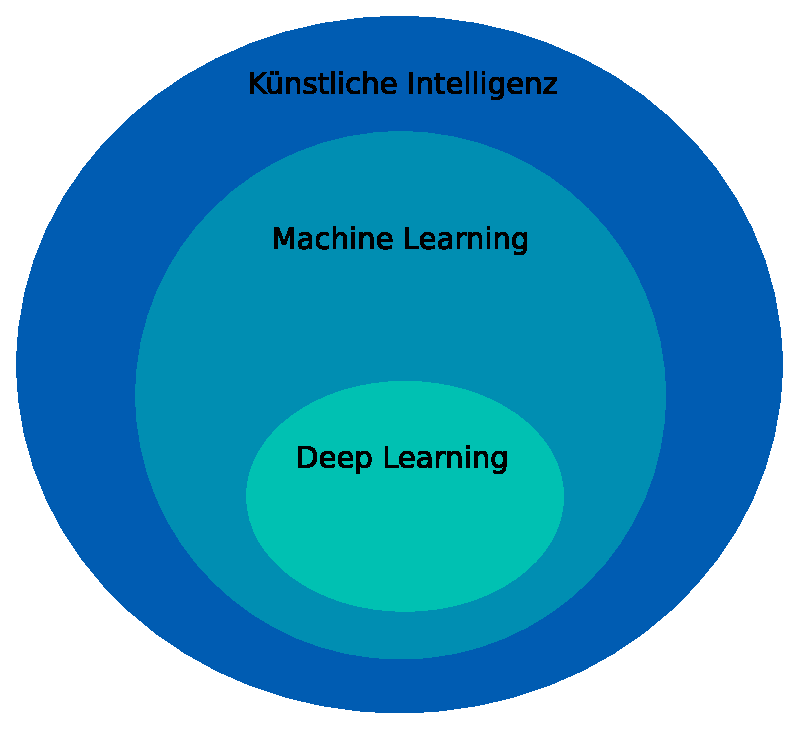
\includegraphics[width = \textwidth]{Pictures/AI.eps}
          \end{minipage}
          \begin{minipage}{0.69 \textwidth}
            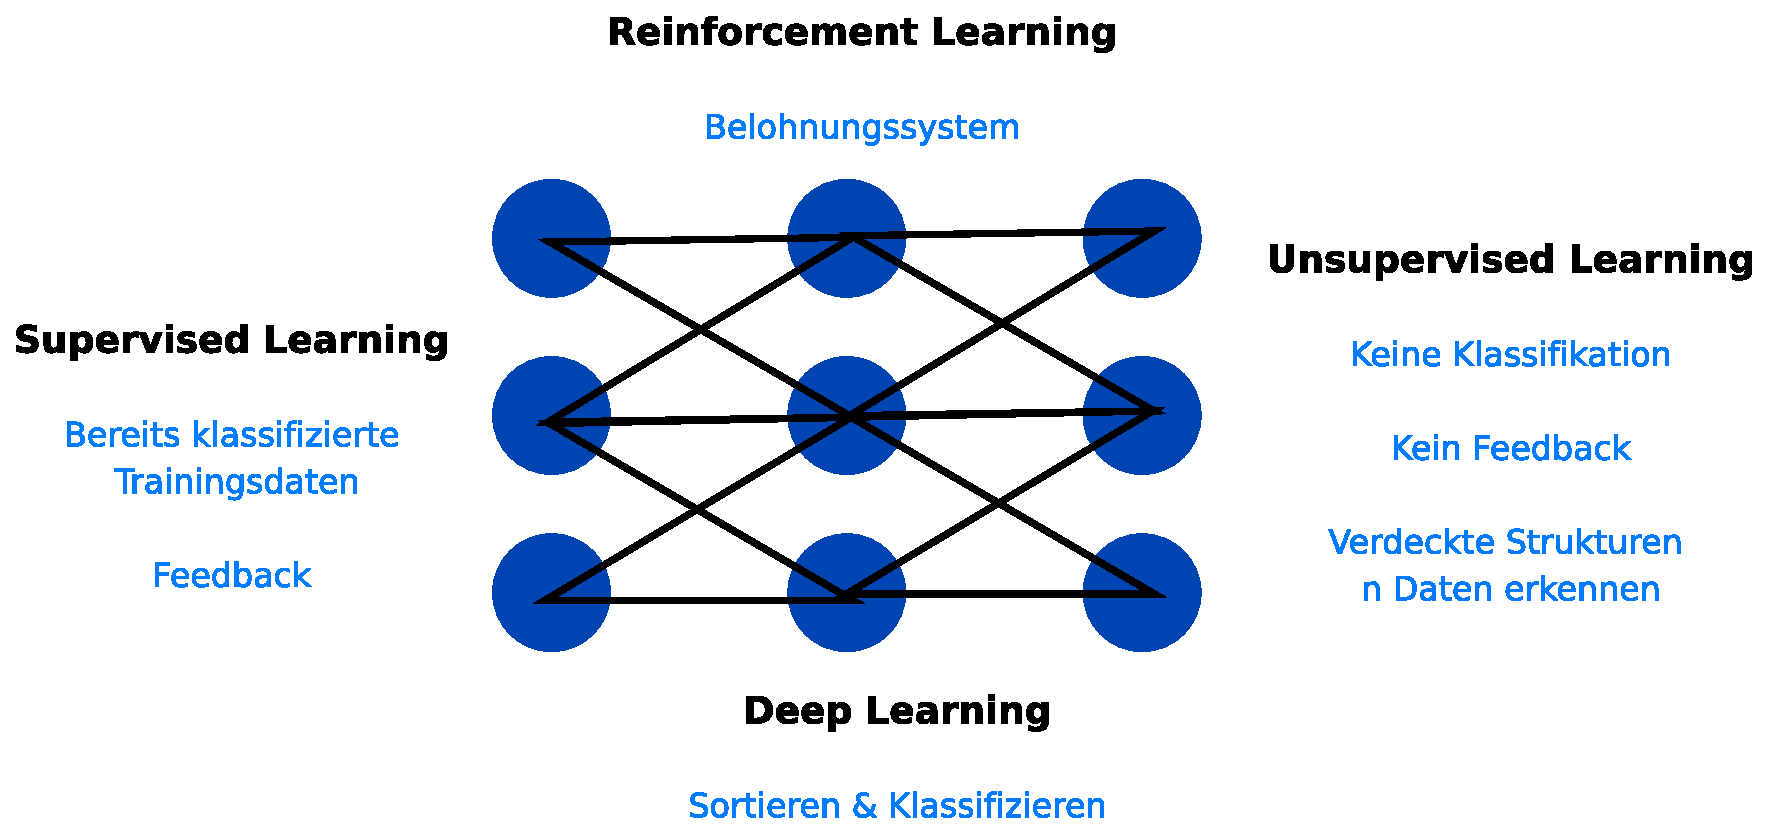
\includegraphics[width = \textwidth]{Pictures/Categories.eps}
          \end{minipage}
        \end{figure}
      }


      \only<5>{
      \framesubtitle{Der Turing Test}
        \begin{figure}
          \begin{minipage}{0.59 \textwidth}
            Methodik von Alan Turing, zur Feststellung menschlichen Verhaltens \cite{TuringTest}
              \begin{itemize}
                \item Entwickelt um 1950
              \end{itemize}
            \end{minipage}
            \begin{minipage}{0.39 \textwidth}
              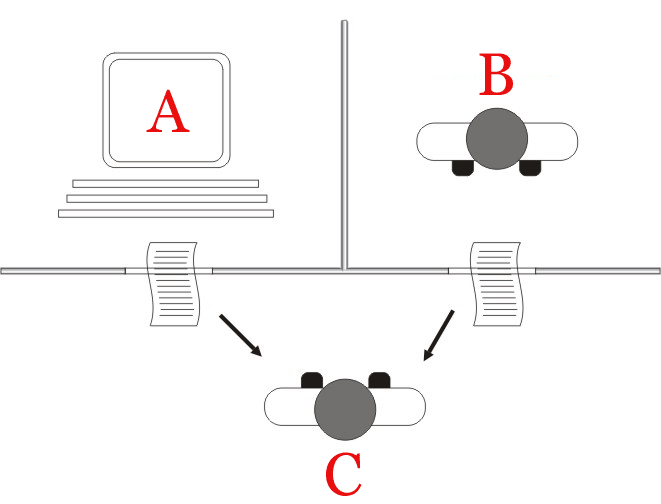
\includegraphics[width = \textwidth]{Pictures/Turing_test_diagram.png}
              \caption{Entnommen von \cite{wiki:Turing_Test}}
            \end{minipage}
          \end{figure}
      }

      \only<6>{
      \framesubtitle{Der Turing Test}
        \begin{figure}
          \begin{minipage}{0.59 \textwidth}
            Methodik von Alan Turing, zur Feststellung menschlichen Verhaltens \cite{TuringTest}
              \begin{itemize}
                \item Entwickelt um 1950 \pause
                \item Relativ simpel \pause
              \end{itemize}
            \end{minipage}
            \begin{minipage}{0.39 \textwidth}
              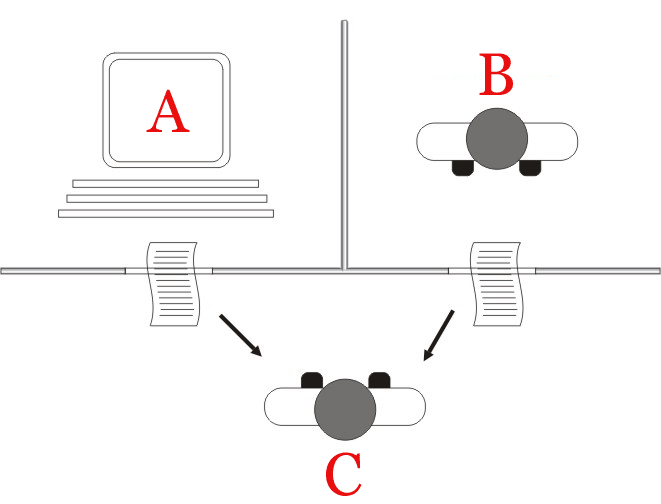
\includegraphics[width = \textwidth]{Pictures/Turing_test_diagram.png}
              \caption{Entnommen von \cite{wiki:Turing_Test}}
            \end{minipage}
          \end{figure}
      }

      \only<7>{
      \framesubtitle{Der Turing Test}
        \begin{figure}
          \begin{minipage}{0.59 \textwidth}
            Methodik von Alan Turing, zur Feststellung menschlichen Verhaltens \cite{TuringTest}
              \begin{itemize}
                \item Entwickelt um 1950
                \item Relativ simpel
                \item Ein Mensch \textbf{C} muss anhand der Antworten die \textbf{A} oder \textbf{B} geben entscheiden welcher Gesprächspartner die KI ist.
              \end{itemize}
            \end{minipage}
            \begin{minipage}{0.39 \textwidth}
              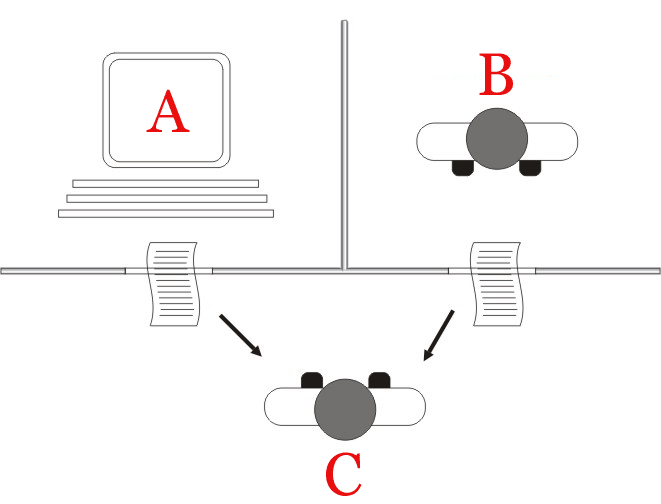
\includegraphics[width = \textwidth]{Pictures/Turing_test_diagram.png}
              \caption{Entnommen von \cite{wiki:Turing_Test}}
            \end{minipage}
          \end{figure}
      }

      \only<8>{
      \framesubtitle{Die Stärke einer KI}
        \begin{center}
          \begin{tabulary}{\textwidth}{C C C}
          \textbf{Starke KI} & $$ \mbox{\huge $ \leftrightarrow $} $$ & \textbf{Schwache KI} \\
          \hline
            Universelle ``Lösungsmaschine'' & & Spezialisiert auf Fachgebiete \\
            & & \\
            Selbstbewusstsein, Emotionen & & Klar zu Lebewesen abgegrenzt \\
            & & \\
            Turing Test nicht auf Aufgabenfeld begrenzt & & meistens enge Anwendungsbereiche\\
            \hline
            \textbf{HAL 9000} & & \textbf{Selbstfahrendes Auto} \\
          \end{tabulary}
        \end{center}
      }

    \end{frame}

    \begin{frame}{Erfindungen einer KI}
      \only<1>{
        \framesubtitle{Die KI als Erfinder?}

        \begin{itemize}
          \item Eine KI ist keine Person, daher kann sie auch kein Erfinder sein

            \item
              \begin{itemize}
                Aktuell können nur natürliche Personen als Erfinder eingetragen werden
            \end{itemize}
        \end{itemize}
      }

      \only<2>{
      \framesubtitle{Die KI als Erfinder?}

      \begin{itemize}
        \item Eine KI ist keine Person, daher kann sie auch kein Erfinder sein
          \item[$ \Rightarrow $] Aktuell können nur natürliche Personen als Erfinder eingetragen werden
        \item Aber: Sobald Mensch involviert, wird die KI als Werkzeug des Menschen angesehen
          \item[$\Rightarrow$] Patent an den Menschen erteilbar
      \end{itemize}
      }

      \only<3>{
        \textbf{Beispiel:}

          Ein Bauteil wurde mithilfe einer KI in einer Weise optimiert die einem Menschen nie eingefallen wäre.
          Das Patent wurde an den Menschen vergeben, da das Bauteil nach §1 PatG eine Erfindung war und die KI als Werkzeug (vergleichbar mit dem Schraubenschlüssel eines Mechanikers) angesehen wurde.
          Relevant ist vor allem dass der Mensch die wesentlichen Entscheidungsschritte getätigt hat.
          \cite{KI_Tagung_DPMA}
      }

    \end{frame}

    \begin{frame}{Patentierbarkeit einer KI}
      \only<1>{
        \framesubtitle{Probleme}
        \begin{itemize}
          \item Grundsätzlich nicht Patentierbar, da Software
          \begin{itemize}
            \item Ausgenommen konkrete Anwendungfälle (siehe Vortrag ``Patentierung von Software'')
          \end{itemize}
        \end{itemize}
      }

      \only<2>{
        \framesubtitle{Probleme}

        \begin{itemize}
          \item Grundsätzlich nicht Patentierbar, da Software
          \begin{itemize}
            \item Ausgenommen sind konkrete Anwendungsfälle (siehe Vortrag ``Patentierung von Software'')
          \end{itemize}
          \item Weiteres Problem: Aktuelle KIs basieren sehr stark auf mathematischen Konzepten
          \begin{itemize}
            \item Auch nicht Patentierbar (vgl. §1 PatG)
          \end{itemize}
        \end{itemize}

      }

      \only<3>{
        \centering
          ``Deep learning'' KIs sind auf eine präzise Auswahl der Trainingsdaten angewiesen, daher kann man sie nur in Kombination mit diesen betrachten
      }

      \only<4>{

        Was mache ich wenn ich meine KI trotzdem schützen will?

      }
      \only <5>{

        \centering

        \textbf{Lösung eine konkreten Technischen Problems mit technischen Mitteln.}\\

        Beispiel: KI eines selbstfahrenden Autos die Kamerabilder für z.B. Verkehrszeichen auswertet. (Aus \cite{KI_DPMA})

      }

      \only <6>{
        \centering
        Hardware Implementierung der KI\\
          \qquad Die spezielle Mikroarchitektur des Prozessors \textbf{kann} durch ein Patent geschützt werden.\\
          \vspace{1 cm}
          \qquad Beispiel: \textbf{DE 20 2019 107 231 U1 - KI-Modul fähig zur Selbstkorrektur unter Zuhilfenahme von Daten und statistischen Operationen} (Siehe \cite{DPARTIS})
      }

    \end{frame}

    \begin{frame}{Fazit}
      \begin{figure}
        \begin{tcolorbox}[colback=green!5,colframe=green!40!black,title=Viele Fragen weiter offen]
            Gerade bei den Referaten aus der unternehmerischen Praxis wurde deutlich, dass die Anwendungen von KI teilweise bereits weit fortgeschritten sind, deren Schutz durch Patente sich aber teilweise noch im Anfangsstadium befindet. Zur Klärung der aufgeworfenen Fragen sind eine weitere intensive Diskussion und die Auslegung der aktuellen Rechtslage durch weitere Urteile der Rechtsprechung notwendig.

            \caption{Entnommen von \url{https://www.dpma.de/dpma/veroeffentlichungen/hintergrund/ki/kki-tagung/index.html}}
        \end{tcolorbox}
      \end{figure}
    \end{frame}

    \begin{frame}{Ende}
        Gibts es Fragen, Anmerkungen, Wünsche?
    \end{frame}

    \bibliography{quote}{}
    \bibliographystyle{plain}
\end{document}
